\section{Design and Theory}
\subsection{Designed velocity Field for planning task}
A velocity field is a function taking as input a state, $q$ and returns a 3-dimensional desired velocity vector $(u,v,w)$.\\ It describes a path (a function of position) as opposed to a trajectory (function of position and time).
\subsubsection{Sink field for reaching the target}
In \cite{mcinnes2003velocity}, the author chose to apply a logarithmic function on the distance between the current position and the goal position as a potential for the sink field. 
However, we observed that using such a potential does not allow the robot to safely approach the goal point since when the distance approaches 0, the logarithmic function diverges.
As a result, we decided to simply use the distance as a potential function. This will allow us to smoothly decrease the velocity of the UAV when approaching the desired goal point.
\subsubsection{Obstacle repulsive field}
In our current solution, because of the simplicity of the environement and the convexity of the obstacles, we are only using the type 1 solution described in \cite{mcinnes2003velocity}, we only have a repulsive field normal to the surface of the obstacle.
\subsubsection{Spherical field to maintain desired force }
When contact has been made, we suppose that the surface static friction coefficient is high enough to maintain the contact.
Since the arm has a fixed size and does not move, this section will describe a velocity field on the surface of a sphere around the target point with a radius defined by the distance between the CoM of the quadcopter and the tip of the arm.\\
First we need to compute the feasible position of the CoM to apply the desired force. 
We know that this position is unique because there is only one vertically stable pitch for a given desired force amplitude. The quadcopter needs to pitch to have a forward velocity because the quadcopter is underactuacted.\\
We can generate the velocity field on the surface of the sphere to point on the tangent direction of the sphere in the direction of the stable pitch position. \\
This field will have an amplitude proportional to the distance from this point.
The planning strategy we described would also allow us to easily define a desirable range for the yaw angle depending on the type of sensor and on the friction coefficient of the target surface.
Finally, we use a Passive Velocity Field Controller \cite{li1999passive} to follow this field to minimize the loss of kinetic energy to the environment when interacting with the surface.
Now we are going to describe how the spherical field is computed. 
Let us recall that the cartesian to spherical coordinate change of variable is defined as
\begin{equation} 
    r = \sqrt{x^2+y^2+z^2}\\ \nonumber 
\end{equation}
\begin{equation}
    \theta = \arccos(\frac{z}{r})\\\nonumber 
\end{equation}
\begin{equation}
    \label{transformation}
    \phi =
    \begin{cases}
        \arctan(\frac{y}{x}), & \text{if $x>0$},\\
        \arctan(\frac{y}{x}) + \pi, & \text{if $x<0$ and $y\geq 0$},\\
        \arctan(\frac{y}{x}) - \pi, & \text{if $x<0$ and $y<0$},\\
        \pi/2, & \text{if $x=0$ and $y>0$},\\
        -\pi/2, & \text{if $x=0$ and $y<0$},\\
        \text{not defined} , & \text{if $x=0$ and $y=0$}
    \end{cases}       
\end{equation}  
The jacobian defining the curvature of the sphere at each point for this transformation is 
\begin{align}
    J = \frac{\partial{(x,y,z)}}{\partial{(r,\phi,\theta)}} \nonumber\\
    J = \begin{bmatrix}
        \sin(\theta)\cos(\phi) & \cos(\theta)\cos(\phi) & -\sin(\phi)\\
        \sin(\theta)\sin(\phi) & \cos(\theta)\sin(\phi) & \cos(\phi)\\
        \cos(\theta) & -\sin(\theta) & 0\\
        \end{bmatrix}
        \label{jacobian}
\end{align}

Figure \ref{fig:spherical} represents an example of such a field where the red point is the optimal position to apply the pressure, the blue arrows are the velocity field vectors and the center of the sphere is the point where the force is applied

\begin{figure*}[h!]
    \centering
    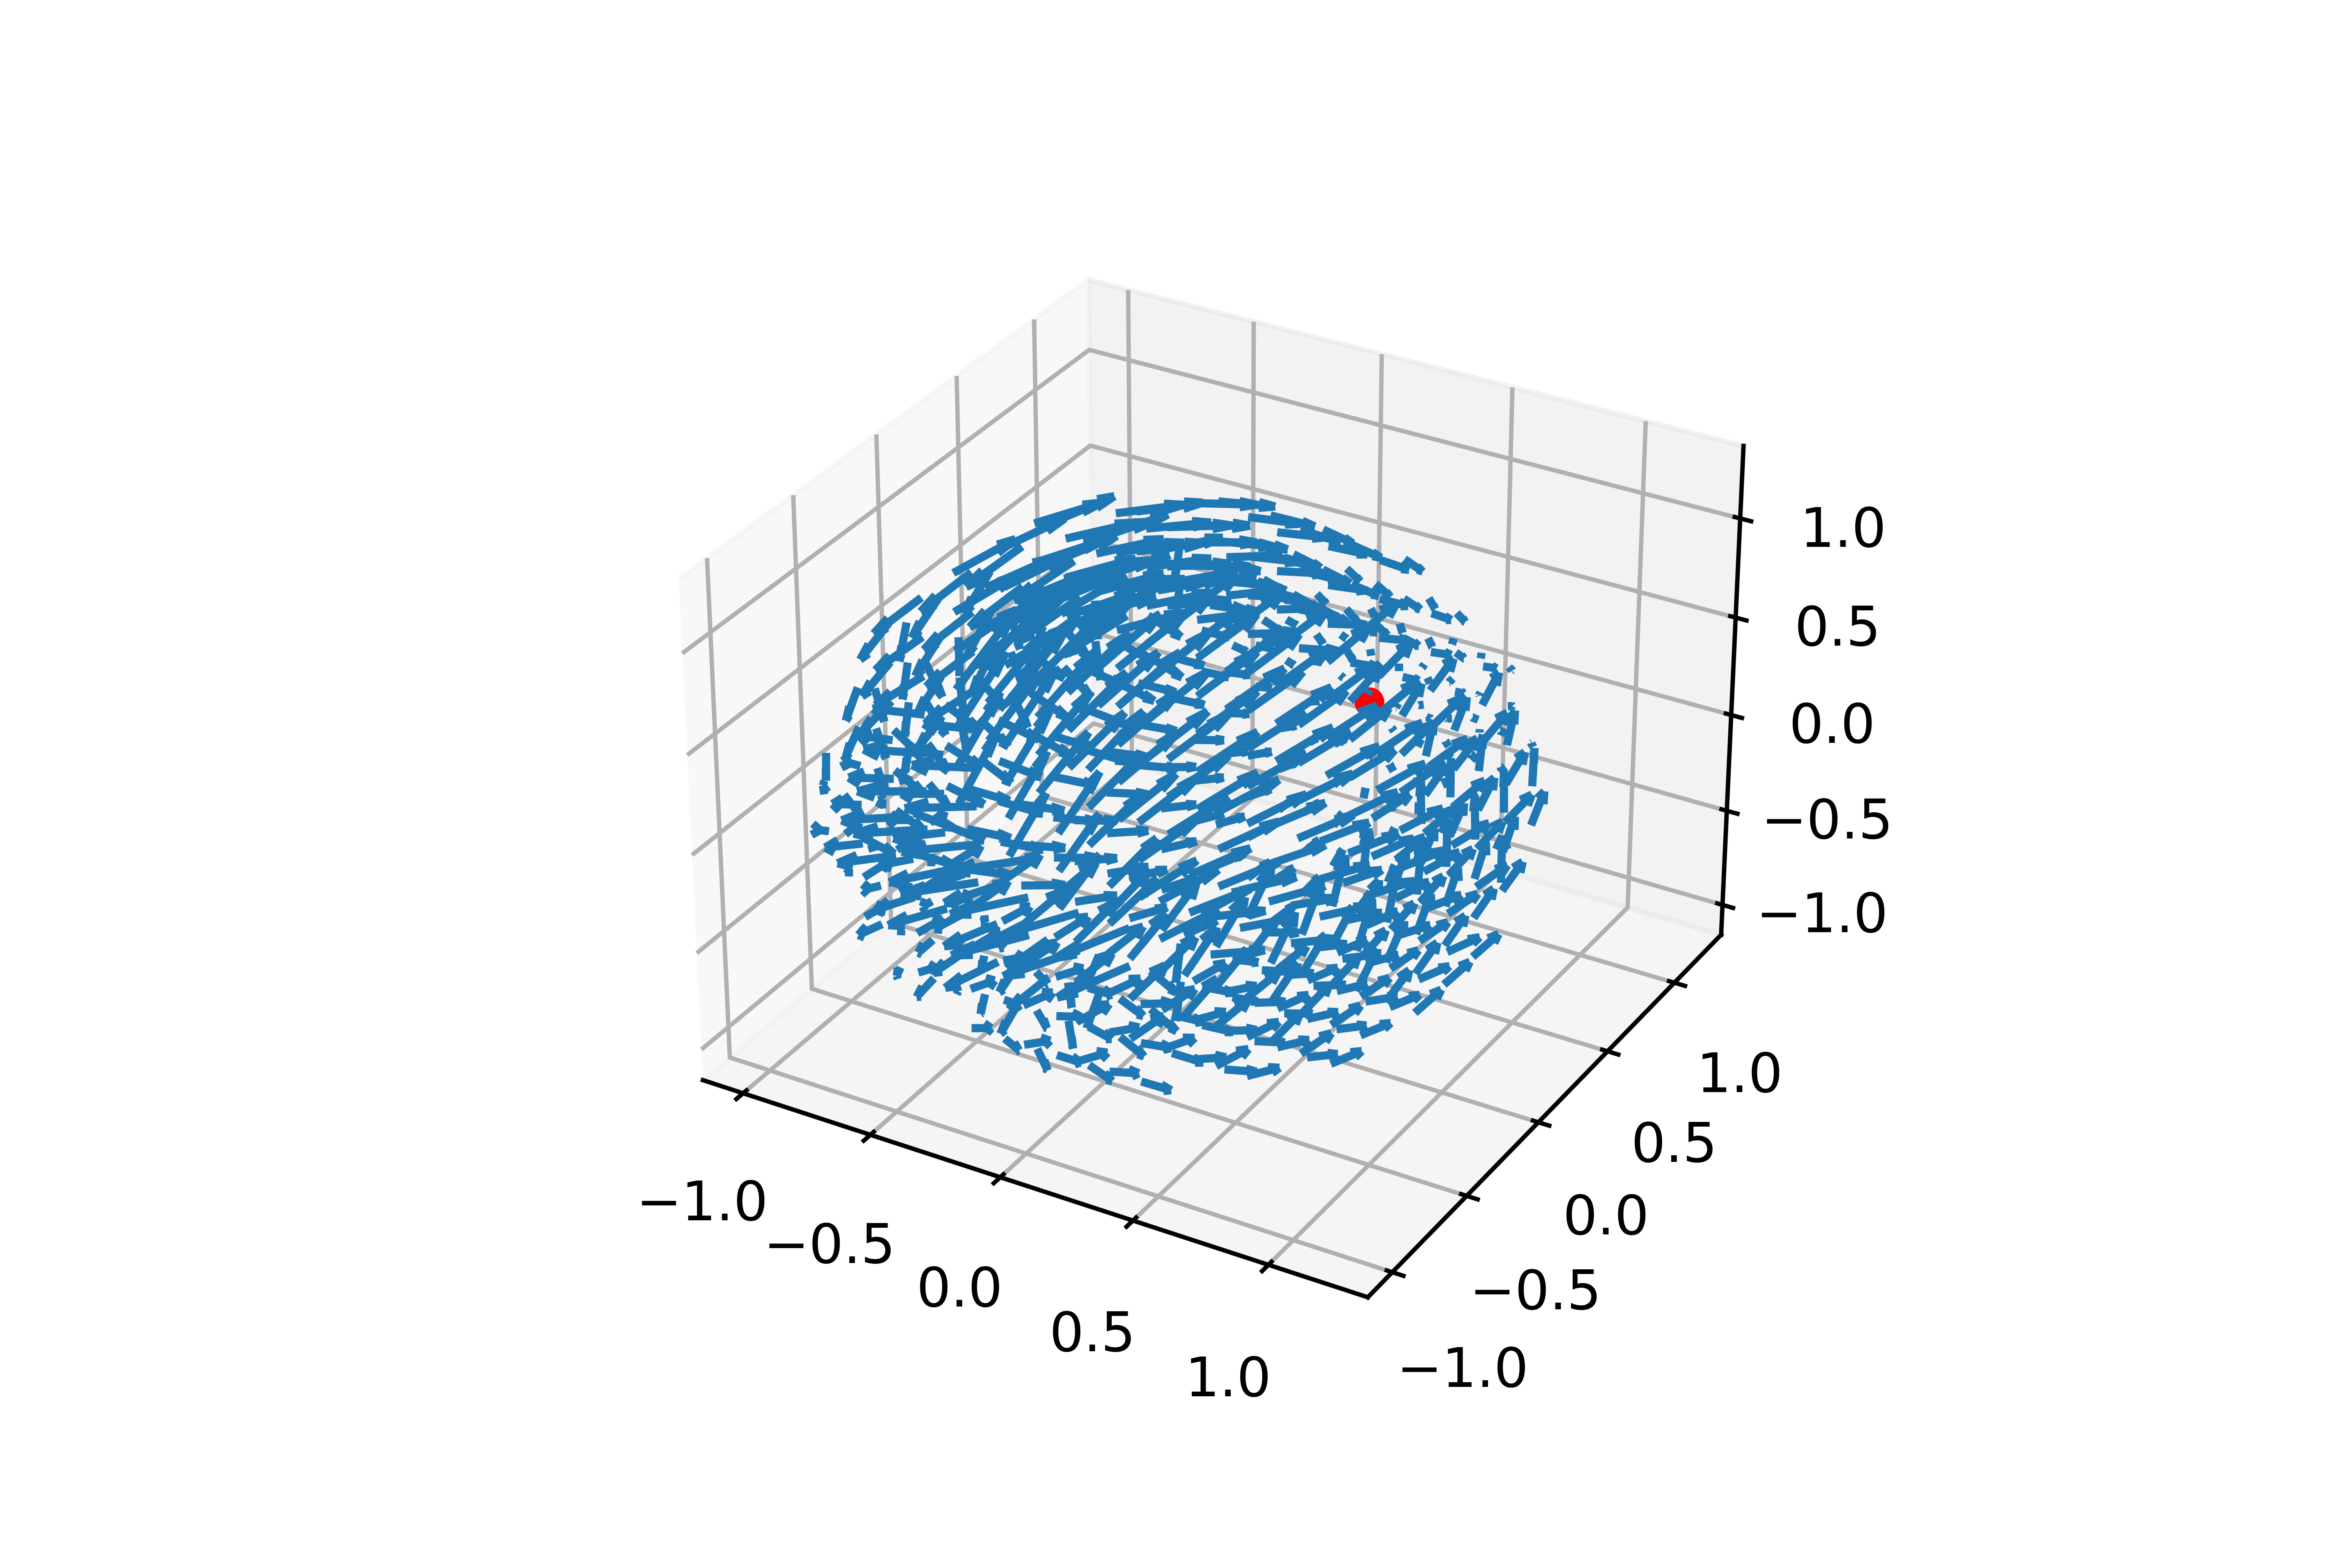
\includegraphics[width=\linewidth]{Images/sphericalfield.png}
    \caption{Spherical contact field}
    \label{fig:spherical}
\end{figure*}
\subsubsection{Circular field for countour following}
This field is based on the methodology explained in \cite{asl2019assistive}. We used it to build intuition, debug and analyze the controller.
The author explains how to encode a countour $\mathcal{C}$ into a desired velocity field $v_d$.
The field is given by: 
\begin{equation}
    v_d(p) = l(\alpha \hat{t} + \lVert Q-p \rVert \hat{n}) \label{eqn:circularfieldcons}
\end{equation}
\begin{itemize}
    \item $p\in \mathbb{R}_3$ is the current position
    \item $Q$ is the closest point from $p$ on $\mathcal{C}$
    \item $l , \alpha \in \mathbb{R}_{\geq 0}$ are scaling constants
    \item $\hat{t}$ is a unitary tangent vector to $\mathcal{C}$ at $Q$
    \item $\hat{n}$ is a unitary normal vector to $\mathcal{C}$ going from $p$ to $Q$
\end{itemize}

\begin{figure}[h!]
    \centering
    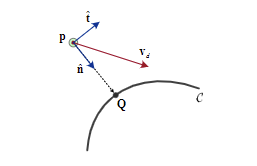
\includegraphics[width=0.48\textwidth]{Images/fieldconstruction.png}
    \caption{field construction from \cite{asl2019assistive}}
    \label{fig:fieldconstruction}
\end{figure} 

From there it is straightforward how to implement a circular velocity field with a radius of 1 and centered at the origin in the following way:
\begin{align}
    Q = \frac{p}{\sqrt{p_x^2 + p_y^2}}\\
    \theta = \arctan(Q_y, Q_x) \\
    \hat{t} = (-\sin{\theta}, \cos{\theta}, 0) \\
    \hat{n} = \frac{Q-p}{\lVert Q-p \rVert}
\end{align}
\subsection{Quadcopter modeling}
\subsubsection{Platform}
Similarly to the platform used in "An Aerial Parallel Manipulator with Shared Compliance", our system is composed of two subsytems: The underactuated quadrotor base (for which we have software in the loop integration given by PX4) and the fixed manipulator arm above the center of mass of the quad.
This system is underactued because in the base frame of this quad, the only thrust direction for the quadcopter is in the $z$ axis in the frame of the base of the quad, the rotors cannot move relative to the base of the quad. Therefore, the IRIS model control inputs are a quarternion vector and a thrust amplitude. However, the output of the passive controller for the non-augmented translational domain is a thrust vector $\Lambda \in\mathbb R_3 $, therefore we will need to convert this desired thrust to the desired format.
In addition to the fixed manipulator arm, a depth camera is mounted on the quad base. We use the depth camera model provided by Pixhawk 4 with IRIS that acts like an intel realsense r200. We use the transform provided in the PX4 obstacle avoidance package to transform from the frame of the camera to the frame of the quadcopter base, and we use the PX4 odometry information to transform from the base to the ground gazebo frame.

\subsubsection{Translational dynamics}

The dynamics that we take into account in our passive control strategy are only in the translational domain. The passive velocity field controller output is a thurst vector and PX4 translates this desired thurst into actual angular velocities for each one of the rotors 
$\Omega = (\bar{\omega_1}, \bar{\omega_2}, \bar{\omega_3}, \bar{\omega_4})$. PVFC only acts on the translational level and not at the rotational level and has no knowledge or control about the speed of thoses rotors and therefore the passivity of this controller is only at the translational level. 
This quadcopter is an underactuacted system because for a given translational velocity, only a subset of attitudes are feasible. As a result, it is not possible to control all 6 degrees of freedom independantly (3 translational, 3 rotational).
 
\subsection{Passive Velocity Field Control of Mechanical Manipulators}
In \cite{li1999passive}, the author explains the advantages of encoding a contour following task using velocity fields. 
They later present the passive velocity field controller whose objective is to "maintain an energetically passive relationship between the manipulator under closed loop control and
its physical environment, while causing the manipulator to perform the desired task." 
We will explain each one of those arguments and relate them to our sensor placement task.
\subsubsection{Velocity fields for planning}
The classical approach to do planning is to encode the task into a timed trajectory $Q:\mathbb R_{\ge 0} \rightarrow G$ where G is the n-dimensional configuration manifold for the manipulator and uses a controller to minimize the state trajectory error.
Using this strategy, the objective of the controller is to minimize the deviation between $q(t)$ and $Q(t)$ where $q:\mathbb R_{\ge 0} \rightarrow G$ is the actual coordinate representation of the manipulator.
This strategy could be fine if the manipulator was able to never deviate from the timed trajectory defined by Q. However, if deviation occurs for example, when external forces are applied to the
robot, a side effect of this minimization strategy called radial reduction can occur.

\begin{figure}[h!]
    \centering
    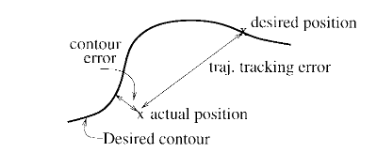
\includegraphics[width=0.48\textwidth]{Images/radialreduction.png}
    \caption{radial reduction from \cite{li1999passive}}
    \label{fig:radialreduction}
\end{figure} 
The author argues that if following the path of the desired trajectory is more important than the timing in which the manipulator follows this trajectory, a strategy based on velocity field is more appropriate because the velocity of the manipulator will only depend on its current position and will be time invariant.  
For the sensor placement task, using a timed trajectory strategy with deviation minimization to reach the contact point may lead the UAV to collide with an obstacle. With our strategy based on potential velocity field, the UAV will not try to shortcut the desired path in case of deviation.
The author defines an $\alpha$ error such that:
\begin{equation}
    e_{\alpha} = \dot{q} - \alpha V \label{alphaerror}
\end{equation}
One of the most important priorities of PVFC is that when no external forces are applied on the robot, there is a positive $\alpha$ such that 
\begin{equation}
    \lim_{t\to\infty}e_{\alpha} = 0
\end{equation}
In other words, PVFC does not seek to exactly match the desired velocity field but just an $\alpha$ scaled version of it. The $\alpha$ we are going to converge to is a function of the energy in the augmented system and the energy in the desired velocity field.
\subsubsection{Passivity}
The controller presented in this paper is based on energy control theory and allows energy transfer between the environement and the augmented system.
Passivity allows dissipation from the energy input to the system into the augmented system. \\
To present this concept, the author first defines the notion of a passive dynamic system:\\
A dynamic system with input $u \in U$ and output $y \in Y$ is passive with respect to the supply rate 
$s:U \cross Y \rightarrow \mathbb R$, if for any $u: \mathbb R_{\ge 0} \rightarrow U $ and for any $t\geq 0$ the following relation is satisfied:
\begin{align}
    \exists ~ c\in\mathbb R  \nonumber\\
    \int_{0}^{t}s(u(\tau),y(\tau))d\tau \geq -c^2 \label{passivityCondition}
\end{align}

Let us remember that the work $W$ and power $P$ of a force $F$ on a point mass object with velocity $v$ are defined as
\begin{align}
    P = F\cdot v\\
    W = \int_{0}^{t}P dt
\end{align}

Therefore the supply rate  $s(\tau_{tot},\dot{q})=\tau_{tot}^{T}\dot{q}$ can be seen as the total mechanical power input. Here the input $\tau_{tot}$ is the total force exerted on the manipulator 
and the output $\dot{q}$ is the velocity of the manipulator. 

When considering a feedback system interacting with the environement shown in figure \ref{fig:pvfccontrolloop}, we can decompose $\tau_{tot}=\tau_{e}+\tau$ (where $\tau$ and $\tau_{e}$ are respectively the forces generated by the actuators and the external forces, for example the contact force when touching a surface),
we can derive the power generated by external forces as $s(\tau_{e}\dot{q})=\tau_{e}^T \dot{q}$. 
\begin{figure}[h!]
    \centering
    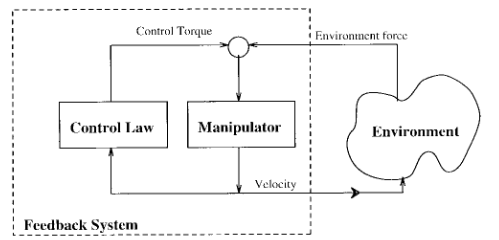
\includegraphics[width=0.48\textwidth]{Images/pvfccontrolloop.png}
    \caption{PVFC loop \cite{li1999passive}}
    \label{fig:pvfccontrolloop}
\end{figure} 
As explained in the paper, a system defined by this supply rate is not passive because obstacles may bring the manipulator to a complete stop for an unbounded amount of time and this loss of kinetic energy cannot be bounded. 
As a result, the passivity relation 
\begin{equation}
    \int_{0}^{t}\tau_{e}^T \dot{q}d\tau \geq -c^2 
\end{equation}
is not valid here because the l.h.s represents the total amount of energy lost to the environment and, as stated before, it cannot be bounded. 
This issue motivates the introduction of an augmented system: a fictitious flywheel is added to the system that acts as an energy storage element.
The dimensionality of the manifold is then increased by one to include the state of the flywheel and this augmented state will be noted as
\begin{align} 
    \bar{q}=[q,q_{\text{fly}}]\\
    \bar{V} = [V, V_{\text{fly}}]
\end{align}

Using such passitive and dissipative systems enables safe interaction between the robot and its environement since the total kinetical energy of the system is bounded by the system initial kinetic energy and energy input from the environement.

\subsubsection{Augmented dynamics}
Let us now describe the dynamics of the augmented system
\begin{equation} 
    \bar{M}(\bar{q})\ddot{\bar{q}} + \bar{C}(\bar{q}, \dot{\bar{q}})\dot{\bar{q}} = \bar{\tau} + \bar{\tau_{e}}
\end{equation}
The mass matrix of the augmented system is defined such that:
\begin{align}
\bar{M}(q) = \begin{bmatrix} 
   M(q) & 0 \\
    0 & m_{\text{fly}}
\end{bmatrix}\\
M(q) =  \begin{bmatrix} 
    m_b & 0 & 0 \\
    0 & m_b & 0 \\
    0 & 0 & m_b \\
 \end{bmatrix}
\end{align}
The Coriolis Matrix of the augmented system is defined such that: 
\begin{align}
\bar{C}(\bar{q}, \dot{\bar{q}}) = \begin{bmatrix} 
    C(q, \dot{q}) & 0 \\
    0 & 0 
\end{bmatrix}
\end{align}
$C$ is built using the Levi–Civita connection described in \cite{li2001passive}.
\subsubsection{Augmented velocity field}
Now let us define the augmented field for the flywheel. The motivation for introducing an augmented system is
to allow energy transfer between the quadcopter actuators and the flywheel such that the total kinetic energy in the system remains constant.
This property is enforced in the definition of the desired velocity field. \\
First let us define $\bar{E}$ to be the total desired energy of the augmented system following the desired velocity field.
$\bar{E}$ can be written as a sum of the flywheel desired kinetic energy $K_{\text{fly}_{d}}$ and the quad desired kinetic energy $K_{quad_{d}}$: 
\begin{equation}
    \bar{E} = K_{\text{fly}_{d}} + K_{quad_{d}}
\end{equation}
Given a desired velocity field $V$ we have: 
\begin{equation}
    K_{quad_{d}}(q) = V(q)^T\frac{1}{2}M(q)V(q)
\end{equation}
Since 
\begin{equation}
    K_{\text{fly}_{d}} = \frac{1}{2} m_{\text{fly}} V^2_{\text{fly}}
\end{equation}
We can derive $V_{\text{fly}}$ in function of  $K_{quad_{d}}(q)$ and $\bar{E}$:
\begin{equation}
    V_{\text{fly}}(q) = \sqrt{\frac{2}{m_{\text{fly}}}(\bar{E}- K_{quad_{d}}(q))} \label{eqn:vfly}
\end{equation}
\subsubsection{PVFC Control law}
To define the PVFC control law, the author defines the following quantities
\begin{align}
    \bar{p}(\bar{q}, \dot{\bar{q}}) = \bar{M}(\bar{q})\dot{\bar{q}} \label{actualaugmomentum}\\
    \bar{P}(\bar{q}) = \bar{M}(\bar{q})\bar{V}(\bar{q}) \label{desiredaugmomentum}\\
    \bar{w}(\bar{q}, \dot{\bar{q}}) = \bar{M}(\bar{q})\dot{\bar{V}} + \bar{C}(\bar{q}, \dot{\bar{q}}) \label{desiredDynamics}
\end{align}
The equation \ref{actualaugmomentum} can be seen as the actual momentum of the augmented system, the equation \ref{desiredaugmomentum} can be seen 
as the desired momentum of the augmented system and \ref{desiredDynamics} is the desired dynamics (desired force applied on) of the augmented system.


From there the author derived the two terms of the coupling control law: 
\begin{align}
    \bar{\tau_c} = \frac{1}{2\bar{E}}(\bar{w}\bar{P}^T - \bar{P}\bar{w}^T ) \dot{\bar{q}} \label{tauc}\\
    \bar{\tau_f} = \gamma(\bar{P}\bar{p}^T - \bar{p}\bar{P}^T ) \dot{\bar{q}} \label{tauf}\\
\end{align}
The anti-symmetric structure of the matrices multiplying $\dot{\bar{q}}$ is key to proving that the derivative of the kinetic energy in the augmented system is: 
\begin{equation}
    \frac{d}{dt}k(\bar{q}, \dot{\bar{q}}) = \tau_e^T(t)\dot{q}(t) \label{kineticdt}
\end{equation}
This is done by introducing the concepts of compatibility between a metric defining an inner product and an affine connection. It is shown in \cite{li2001passive} that the compatibility between the Levi-Civita connection with the metric defined by $M$ has a direct link between anti-symmetricity of the matrices in the control coupling law, passivity and energy conservation.

From equations \ref{kineticdt} and \ref{passivityCondition}, the passivity of the system with respect to external forces is straightforward.

\subsection{Compensation terms}
When using PVFC with the quadcopter dynamics, it is important to model the effect of drag and gravity on the robot to be able to compensate for them. If those forces are not taken into account, the robot total mechanical energy will decrease until it arrives to a complete stop. 
Therefore, to ensure the robot will continue to follow the desired velocity field, we have to introduce compensation terms for gravity and air drag. 
For simplicity, we chose to model drag as a linear function of the velocity. This worked for our proof of concept but this method 
shows its limits when running the simulation for a greater amount of time because not only drag is not exactly proportional to the speed, but we have no straightforward way of estimating those drag coefficients.
Setting them too high will make our control ouput diverge but setting it too low will make to quad stop following the desired velocity field.  
